\newif\ifglobal

%%%%%%%%%%%%%%%%%%%%%%%
%%% Compile to view %%%
%%%%%%%%%%%%%%%%%%%%%%%

%%%%%%%%%%%%%%%%%%%%%%%%%%%%%%%%%%%%%%%%%%%%%%%%%%%
%%% Readme:                                     %%%
%%% https://www.overleaf.com/read/bwdjvfjksvjy/ %%%
%%%%%%%%%%%%%%%%%%%%%%%%%%%%%%%%%%%%%%%%%%%%%%%%%%%

% >>> M?: marks a module setting number or important notice

% >>> M4: Set {./relative-path} to external files for this module <<<
\def \modulefiles {./52-LEDPWM}
% To add an external file, use:
% (Replace '---' with actual filename)
% '\input{\modulefiles/tables/---.tex}' for tables
% '\includegraphics{\modulefiles/figures/---}' for figures
% '\subfile{\modulefiles/---}' for register files

% >>> M1: This module is in global project? <<<
% 'YES' - uncomment; 'NO' - comment out
\globaltrue

\ifglobal
    \documentclass[main\_\_EN.tex]{subfiles}
   
\else
    \documentclass[openany, 10pt]{book}

    % >>> M2: In ./00-shared/preamble-trm-module, also find
    %         settings for visibility of todo notes, watermark <<<
    \usepackage{preamble-trm-module}

    % >>> M3: Temporary labels in English,
    %         you can add your own labels there <<<
    \myexternaldocument{./00-shared/temp-labels-en}

\fi %\ifglobal


\setcounter{secnumdepth}{4}


% >>> M5: If this module needs any updates in
% './00-shared/preamble-trm-module.sty'
% (include additional package, etc.), contact your module PM
% or create the file './00-shared/changelog.tex' make the
% necessary updates yourself and document them in this file <<<

% Make text left-aligned and allow latex to break pages naturally, comment out for full justification
\raggedright
\raggedbottom


\begin{document}


% Sets language into which pre-defined bits of text are translated
\selectlanguage{english}
\setenglishformatting

% Do not delete this block
\ifglobal
% Add the following front matter if
% this module is outside of global project
\else
    \InputIfFileExists{readme}{}{}
    \clearpage
    \listoftodos
    \listofdonetodos
    \tableofcontents
    %\listoftables
    %\listoffigures
\fi


%%%%%%%%%%%%%%%%%%%%%%%%%
%%% TRM Module Begins %%%
%%%%%%%%%%%%%%%%%%%%%%%%%

\hypertarget{ledpwm}{}
\chapter{LED PWM Controller (LEDC)}
\label{mod:ledpwm}

\section{Overview}

The LED PWM Controller is a peripheral designed to generate pulse-width modulation (PWM) signals for LED control. It has specialized features such as automatic duty cycle fading, and can also be used to generate PWM signals for other purposes.

\section{Features}
The LED PWM Controller has the following features:
\begin{itemize}
    \item Two independent LED PWM controllers (LEDC0, LEDC1), each containing 8 independent PWM generation channels (16 channels in total)
    \item Maximum PWM duty cycle resolution: 20 bits
    \item Four independent timers per LED PWM controller, supporting fractional division
    \item Adjustable phase of PWM signal output
    \item PWM duty cycle dithering
    \item Automatic duty cycle fading \textendash\ gradual increase or decrease of a PWM's duty cycle without processor intervention. An interrupt is generated upon fade completion
    \item Up to 16 duty cycle ranges for each PWM generator to generate gamma curve signals \textendash\ each range can be independently configured in terms of fading direction, the step size, the number of fades, and the fading frequency
    \item PWM signal output in low-power mode (Light-sleep mode)
    \item Event generation and task response managed by the Event Task Matrix (ETM) peripheral
\end{itemize}

The two independent LED PWM controllers are identical. The following sections describe one of them as an example.

Note that the four timers are identical regarding their features and operation. The following sections refer to the timers collectively as Timer\regindex{x} (where \regindex{x} ranges from 0 to 3). Likewise, the eight PWM generators are also identical in features and operation, and thus are collectively referred to as PWM\regindex{n} (where \regindex{n} ranges from 0 to 7).

%%%%%%%%%%%%%%%%%%%%%%%%%%%%%%
%%% Architectural Overview %%%
%%%%%%%%%%%%%%%%%%%%%%%%%%%%%%

\section{Architectural Overview}
\label{sec:ledc-arch-overview}

Figure \ref{fig:ledc-architecture} shows the architecture of the LED PWM Controller.

    \begin{figure}[H]
        \centering
        
\includegraphics[width=0.6\textwidth]{\modulefiles/figures/led2-1_912}
        \caption{LED PWM Architecture}
        \label{fig:ledc-architecture}
    \end{figure}

Each of the four timers has an internal timebase counter (i.e., a counter that counts on cycles of a reference clock) and thus can be independently configured (i.e., configurable clock divider, and counter overflow value). Each PWM generator selects one of the four timers by configuring the \hyperref[fielddesc:LEDCTIMERSELCHN]{LEDC\_TIMER\_SEL\_CH\regindex{n}}, and uses the timer's counter value timer\regindex{x}\_cnt as a reference to generate its PWM signal.

Figure \ref{fig:ledc-pwm-generator} illustrates the main functional blocks of the timer and the PWM generator.

    \begin{figure}[H]
        \centering
        
\includegraphics[width=1.0\textwidth]{\modulefiles/figures/ledc_2-2}
        \caption{Timer and PWM Generator Block Diagram}
        \label{fig:ledc-pwm-generator}
    \end{figure}

\section{Functional Description}

\subsection{Clock}
The LED PWM Controller uses two types of clocks:

\begin{itemize}
    \item APB\_CLK: bus clock used to configure LED PWM registers
    \item LEDC0/1\_CLK: function clock for the LED PWM Controller to operate
\end{itemize}

\begin{figure}[H]
    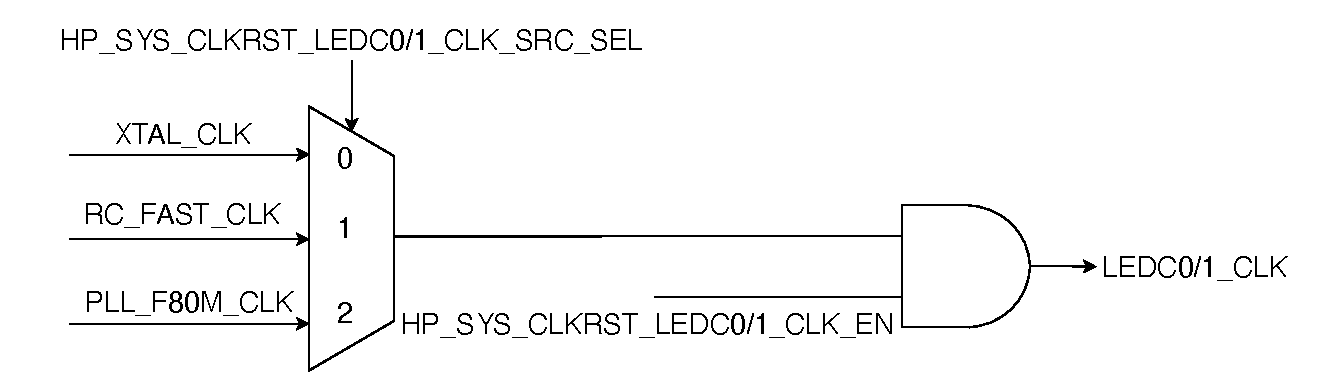
\includegraphics[width=0.8\linewidth]{52-LEDPWM/figures/ledc_clk.pdf}
    \centering
    \caption{LEDC\_CLK Diagram}
    \label{fig:module-clk}
\end{figure}

As shown in \ref{fig:module-clk} \textit{\nameref{fig:module-clk}}, the function clock LEDC\_CLK can be sourced from:

\begin{itemize}
    \item XTAL\_CLK
    \item RC\_FAST\_CLK
    \item PLL\_F80M\_CLK
\end{itemize}


For more information on clocks, see Chapter \ref{mod:resclk} \textit{\nameref{mod:resclk}}.

For detailed clock programming procedures, see Section \ref{sec:ledc-prog-procedures} \textit{\nameref{sec:ledc-prog-procedures}}.

\subsection{Reset}

The LED PWM Controller can be fully reset by setting the \hyperref[fielddesc:HPSYSCLKRSTLEDC0RSTEN]{HP\_SYS\_CLKRST\_LEDC0\_RST\_EN} or  \hyperref[fielddesc:HPSYSCLKRSTLEDC1RSTEN]{HP\_SYS\_CLKRST\_LEDC1\_RST\_EN} fields in the \hyperref[regdesc:HPSYSCLKRSTLEDCCTRL0REG]{HP\_SYS\_CLKRST\_LEDC\_CTRL0\_REG} register.

\subsection{Timers}\label{sec:ledc-timers}

Each timer in the LED PWM Controller internally maintains a timebase counter. Referring to Figure \ref{fig:ledc-pwm-generator}, the clock signal used by the timebase counter is named ref\_pulse\regindex{x}. All timers use the same clock source, LEDC\_CLK, which is then passed through a clock divider to generate ref\_pulse\regindex{x} for the counter. Each timer can be independently enabled by setting the corresponding \hyperref[fielddesc:LEDCTIMERXPOWERUP]{LEDC\_TIMER\regindex{x}\_POWER\_UP} field, and disabled by clearing the corresponding \hyperref[fielddesc:LEDCTIMERXPOWERUP]{LEDC\_TIMER\regindex{x}\_POWER\_UP} field.

\subsubsection{Clock Divider Configuration}

The LEDC\_CLK signal is passed through a clock divider to generate the ref\_pulse\regindex{x} signal for the counter. The frequency of ref\_pulse\regindex{x} is equal to the frequency of LEDC\_CLK divided by the divisor LEDC\_CLK\_DIV (see Figure \ref{fig:ledc-pwm-generator}).

The clock divider is a fractional divider. Thus, the divisor LEDC\_CLK\_DIV can be a non-integer value. LEDC\_CLK\_DIV is configured according to the following equation.

\begin{center}
$\textrm{LEDC\_CLK\_DIV} = A + \frac{B}{256}$
\end{center}

\begin{itemize}
    \item The integer part \textit{A} corresponds to the most significant 10 bits of \hyperref[fielddesc:LEDCCLKDIVTIMERX]{LEDC\_CLK\_DIV\_TIMER\regindex{x}} (i.e., \hyperref[regdesc:LEDCTIMERXCONFREG]{LEDC\_TIMER\regindex{x}\_CONF\_REG}[22:13])
    \item The fractional part \textit{B} corresponds to the least significant 8 bits of \hyperref[fielddesc:LEDCCLKDIVTIMERX]{LEDC\_CLK\_DIV\_TIMER\regindex{x}} \\(i.e., \hyperref[regdesc:LEDCTIMERXCONFREG]{LEDC\_TIMER\regindex{x}\_CONF\_REG}[12:5])
\end{itemize}

When the fractional part \textit{B} is 0, LEDC\_CLK\_DIV is equivalent to an integer divisor (i.e., an integer prescaler). In other words, a ref\_pulse\regindex{x} clock pulse is generated after every \textit{A} number of LEDC\_CLK clock pulses.

However, when \textit{B} is not 0, LEDC\_CLK\_DIV becomes a non-integer divisor. The clock divider implements non-integer frequency division by alternating between \textit{A} and (\textit{A}+1) LEDC\_CLK clock pulses per ref\_pulse\regindex{x} clock pulse. In this way, the average frequency of ref\_pulse\regindex{x} clock pulse will be the desired frequency (i.e., the non-integer divided frequency). For every 256 ref\_pulse\regindex{x} clock pulses:

\begin{itemize}
    \item A number of \textit{B} ref\_pulse\regindex{x} clock pulses are generated every (\textit{A}+1) LEDC\_CLK clock pulses
    \item A number of (256-\textit{B}) ref\_pulse\regindex{x} clock pulses are generated every \textit{A} LEDC\_CLK clock pulses
    \item The ref\_pulse\regindex{x} clock pulses generated every (\textit{A}+1) pulses are evenly distributed amongst those generated every \textit{A} pulses
\end{itemize}

Figure \ref{fig:ledc-divider} illustrates the relation between LEDC\_CLK clock pulses and ref\_pulse\regindex{x} clock pulses when LEDC\_CLK\_DIV is a non-integer value.

\begin{figure}[ht]
    \centering
    \fbox{
\includegraphics[width=1\textwidth]{\modulefiles/figures/ledc_frag_div}}
    \caption{Frequency Division When LEDC\_CLK\_DIV is a Non-Integer Value}
    \label{fig:ledc-divider}
\end{figure}

To change the timer's clock divisor at runtime, first configure the \hyperref[fielddesc:LEDCCLKDIVTIMERX]{LEDC\_CLK\_DIV\_TIMER\regindex{x}} field, and then set the \hyperref[fielddesc:LEDCTIMERXPARAUP]{LEDC\_TIMER\regindex{x}\_PARA\_UP} field to apply the new configuration. This will cause the newly configured values to take effect upon the next overflow of the counter. The \hyperref[fielddesc:LEDCTIMERXPARAUP]{LEDC\_TIMER\regindex{x}\_PARA\_UP} field will be automatically cleared by hardware.

\subsubsection{20-Bit Counter}

Each timer contains a 20-bit timebase counter that uses ref\_pulse\regindex{x} as its reference clock (see Figure \ref{fig:ledc-pwm-generator}). The \hyperref[fielddesc:LEDCTIMERXDUTYRES]{LEDC\_TIMER\regindex{x}\_DUTY\_RES} field configures the actual used bit width of this 20-bit counter. Hence, the maximum resolution of the PWM signal is 20 bits. The counter counts up to $2^{\textrm{\hyperref[fielddesc:LEDCTIMERXDUTYRES]{LEDC\_TIMER\regindex{x}\_DUTY\_RES}}}-1$, overflows and begins counting from 0 again. The counter's value can be read, reset, and suspended by software. Figure \ref{fig:ledc-res} shows the relationship between the counter and PWM resolution.

\begin{figure}[ht]
    \centering
    \fbox{
\includegraphics[width=1\textwidth]{\modulefiles/figures/ledc_res}}
    \caption{Relationship Between Counter And Resolution}
    \label{fig:ledc-res}
\end{figure}

Every time the counter overflows, it can trigger the \hyperref[int:ledc-timer-ovf]{LEDC\_TIMER\regindex{x}\_OVF\_INT} interrupt (generated automatically by hardware without configuration). It can also be configured to trigger \hyperref[int:ledc-ovf-cnt]{LEDC\_OVF\_CNT\_CH\regindex{n}\_INT} after overflowing $\textrm{\hyperref[fielddesc:LEDCOVFNUMCHN]{LEDC\_OVF\_NUM\_CH\regindex{n}} + 1}$ times. To configure \hyperref[int:ledc-ovf-cnt]{LEDC\_OVF\_CNT\_CH\regindex{n}\_INT} interrupt, please:

 \begin{enumerate}
    \item Configure \hyperref[fielddesc:LEDCTIMERSELCHN]{LEDC\_TIMER\_SEL\_CH\regindex{n}} to select the timer for the PWM generator
    \item Enable the overflow counter by setting  \hyperref[fielddesc:LEDCOVFCNTENCHN]{LEDC\_OVF\_CNT\_EN\_CH\regindex{n}}
    \item Configure \hyperref[fielddesc:LEDCOVFNUMCHN]{LEDC\_OVF\_NUM\_CH\regindex{n}} with the number of counter overflows (that triggers an interrupt) minus 1
    \item Enable the overflow interrupt by setting \hyperref[fielddesc:LEDCOVFCNTCHNINTENA]{LEDC\_OVF\_CNT\_CH\regindex{n}\_INT\_ENA}
    \item Configure \hyperref[fielddesc:LEDCTIMERXDUTYRES]{LEDC\_TIMER\regindex{x}\_DUTY\_RES} to specify the counter bit width for the selected Timer\regindex{x} and wait for a \hyperref[int:ledc-ovf-cnt]{LEDC\_OVF\_CNT\_CH\regindex{n}\_INT} interrupt
\end{enumerate}

To change the overflow value at runtime, first set the \hyperref[fielddesc:LEDCTIMERXDUTYRES]{LEDC\_TIMER\regindex{x}\_DUTY\_RES} field, and then set the\\ \hyperref[fielddesc:LEDCTIMERXPARAUP]{LEDC\_TIMER\regindex{x}\_PARA\_UP} field. This will cause the newly configured values to take effect upon the next overflow of the counter. If \hyperref[fielddesc:LEDCOVFCNTENCHN]{LEDC\_OVF\_CNT\_EN\_CH\regindex{n}} field is reconfigured, \hyperref[fielddesc:LEDCPARAUPCHN]{LEDC\_PARA\_UP\_CH\regindex{n}} should be set to apply the new configuration. In summary, these configuration values need to be updated by setting \hyperref[fielddesc:LEDCTIMERXPARAUP]{LEDC\_TIMER\regindex{x}\_PARA\_UP} or \hyperref[fielddesc:LEDCPARAUPCHN]{LEDC\_PARA\_UP\_CH\regindex{n}}. \hyperref[fielddesc:LEDCTIMERXPARAUP]{LEDC\_TIMER\regindex{x}\_PARA\_UP} and \hyperref[fielddesc:LEDCPARAUPCHN]{LEDC\_PARA\_UP\_CH\regindex{n}} will be automatically cleared by hardware.

Referring to Figure \ref{fig:ledc-pwm-generator}, the frequency of a PWM generator output signal (sig\_out\regindex{n}) is dependent on the frequency of the timer's clock source LEDC\_CLK, the clock divisor LEDC\_CLK\_DIV, and the duty resolution (counter width) \hyperref[fielddesc:LEDCTIMERXDUTYRES]{LEDC\_TIMER\regindex{x}\_DUTY\_RES}:

    \[
    f_{\textrm{PWM}}=\frac{f_{\textrm{LEDC\_CLK}}}
                        {\textrm{LEDC\_CLK\_DIV}\cdot 2^{\textrm{\hyperref[fielddesc:LEDCTIMERXDUTYRES]{LEDC\_TIMER\regindex{x}\_DUTY\_RES}}}}
    \]

Based on the formula above, the desired duty resolution can be calculated as follows:

    \[
    \textrm{\hyperref[fielddesc:LEDCTIMERXDUTYRES]{LEDC\_TIMER\regindex{x}\_DUTY\_RES}}
    =\log_2\left(\frac{f_{\textrm{LEDC\_CLK}}}
    {f_{\textrm{PWM}}\cdot \textrm{LEDC\_CLK\_DIV}}\right)
    \]


Table \ref{tab:ledc-common-freq-res} lists the commonly-used frequencies and their corresponding resolutions.

\begin{ThreePartTable}

    \begin{TableNotes}

        \item[1] The highest resolution is calculated when the clock divisor LEDC\_CLK\_DIV is 1. If the highest resolution calculated by the formula is higher than the counter's width 20 bits, then the highest resolution should be 20 bits.

        \item[2] The lowest resolution is calculated when the clock divisor LEDC\_CLK\_DIV is $1023+\frac{255}{256}$. If the lowest resolution calculated by the formula is lower than 0, then the lowest resolution should be 1.

    \end{TableNotes}

\begin{longtable}[c]{ | l | l | l | l | }
\caption{Commonly-used Frequencies and Resolutions}
\label{tab:ledc-common-freq-res}
\\\hline
\rowcolor{lightgray}
LEDC\_CLK & PWM Frequency & Highest Resolution (bit) \tnote{1} & Lowest Resolution (bit) \tnote{2} \\\hline

\endhead
\insertTableNotes
\endlastfoot

REF\_80M\_CLK (80 MHz) & 1 kHz & 16 & 7 \\\hline
REF\_80M\_CLK (80 MHz) & 5 kHz & 13 & 4 \\\hline
REF\_80M\_CLK (80 MHz) & 10 kHz & 12 & 3 \\\hline
XTAL\_40M\_CLK (40 MHz) & 1 kHz & 15 & 6 \\\hline
XTAL\_40M\_CLK (40 MHz) & 4 kHz & 13 & 4 \\\hline
FOSC\_20M\_CLK (20 MHz) & 1 kHz & 14 & 5 \\\hline
FOSC\_20M\_CLK (20 MHz) & 2 kHz & 13 & 4 \\\hline
\end{longtable}
\end{ThreePartTable}

\subsubsection{Timer Configuration Constraints}

The clock divisor LEDC\_CLK\_DIV and the duty resolution \hyperref[fielddesc:LEDCTIMERXDUTYRES]{LEDC\_TIMER\regindex{x}\_DUTY\_RES} of the timer's 20-bit counter must satisfy the following condition:

\begin{equation}
    {\textrm{LEDC\_CLK\_DIV}\cdot 2^{\textrm{\hyperref[fielddesc:LEDCTIMERXDUTYRES]{LEDC\_TIMER\regindex{x}\_DUTY\_RES}}}} \ge 8
\end{equation}

\subsection{PWM Generators}\label{sec:ledc-pwm-generator}

Each LED PWM generator can be independently enabled by setting the corresponding \hyperref[fielddesc:LEDCCHNPOWERUP]{LEDC\_CH\regindex{n}\_POWER\_UP} field.

To generate a PWM signal, a PWM generator (PWM\regindex{n}) needs a timer (Timer\regindex{x}). Each PWM generator can be configured separately by setting \hyperref[fielddesc:LEDCTIMERSELCHN]{LEDC\_TIMER\_SEL\_CH\regindex{n}} to use one of four timers to generate the PWM output.

As shown in Figure \ref{fig:ledc-pwm-generator}, each PWM generator mainly consists of a comparator and two multiplexers. A PWM generator compares the timer's 20-bit counter value (Timer\regindex{x}\_cnt) to two trigger values Hpoint\regindex{n} and Lpoint\regindex{n}. When the timer's counter value is equal to Hpoint\regindex{n} or Lpoint\regindex{n}, the PWM signal can output a high or low level:

\begin{itemize}
\item If Timer\regindex{x}\_cnt == Hpoint\regindex{n}, sig\_out\regindex{n} is 1.
\item If Timer\regindex{x}\_cnt == Lpoint\regindex{n}, sig\_out\regindex{n} is 0.
\end{itemize}

Figure \ref{fig:ledc-fixed-duty} illustrates how Hpoint\regindex{n} and Lpoint\regindex{n} are used to generate a fixed duty cycle PWM output signal.

\begin{figure}[ht]
    \centering
    \fbox{
\includegraphics[width=1\textwidth]{\modulefiles/figures/ledc_2-3_761}}
    \caption{LED PWM Output Signal Diagram}
    \label{fig:ledc-fixed-duty}
\end{figure}

For a particular PWM generator (PWM\regindex{n}), its Hpoint\regindex{n} is sampled from the \hyperref[fielddesc:LEDCHPOINTCHN]{LEDC\_HPOINT\_CH\regindex{n}} field each time the selected timer's counter overflows. Likewise, Lpoint\regindex{n} is also sampled on every counter overflow and is calculated from the sum of the \hyperref[fielddesc:LEDCDUTYCHN]{LEDC\_DUTY\_CH\regindex{n}}[24:4] and \hyperref[fielddesc:LEDCHPOINTCHN]{LEDC\_HPOINT\_CH\regindex{n}} fields. By setting Hpoint\regindex{n} and Lpoint\regindex{n} via the \hyperref[fielddesc:LEDCHPOINTCHN]{LEDC\_HPOINT\_CH\regindex{n}} and \hyperref[fielddesc:LEDCDUTYCHN]{LEDC\_DUTY\_CH\regindex{n}}[24:4] fields, the relative phase and duty cycle of the PWM output can be set.

The PWM output signal (sig\_out\regindex{n}) is enabled by setting \hyperref[fielddesc:LEDCSIGOUTENCHN]{LEDC\_SIG\_OUT\_EN\_CH\regindex{n}}. When \hyperref[fielddesc:LEDCSIGOUTENCHN]{LEDC\_SIG\_OUT\_EN\_CH\regindex{n}} is cleared, PWM signal output is disabled, and the output signal (sig\_out\regindex{n}) will output a constant level specified by \hyperref[fielddesc:LEDCIDLELVCHN]{LEDC\_IDLE\_LV\_CH\regindex{n}}.

\subsubsection{PWM Output Signal Dithering}
The bits \hyperref[fielddesc:LEDCDUTYCHN]{LEDC\_DUTY\_CH\regindex{n}}[3:0] are used to dither the duty cycles of the PWM output signal (sig\_out\regindex{n}) by periodically altering the duty cycle of sig\_out\regindex{n}. When \hyperref[fielddesc:LEDCDUTYCHN]{LEDC\_DUTY\_CH\regindex{n}}[3:0] is not 0, then for every 16 cycles of sig\_out\regindex{n}, \hyperref[fielddesc:LEDCDUTYCHN]{LEDC\_DUTY\_CH\regindex{n}}[3:0] of those cycles will have PWM pulses that are one timer tick longer than the other (16 – \hyperref[fielddesc:LEDCDUTYCHN]{LEDC\_DUTY\_CH\regindex{n}}[3:0]) cycles. For instance, if \hyperref[fielddesc:LEDCDUTYCHN]{LEDC\_DUTY\_CH\regindex{n}}[24:4] is set to 10 and \hyperref[fielddesc:LEDCDUTYCHN]{LEDC\_DUTY\_CH\regindex{n}}[3:0] is set to 5, then 5 of 16 cycles will have a PWM pulse with a duty value of 11 and the rest of the 16 cycles will have a PWM pulse with a duty value of 10. The average duty cycle after 16 cycles is 10.3125.

\subsubsection{Applying the Changed Configuration}
If fields \hyperref[fielddesc:LEDCTIMERSELCHN]{LEDC\_TIMER\_SEL\_CH\regindex{n}}, \hyperref[fielddesc:LEDCHPOINTCHN]{LEDC\_HPOINT\_CH\regindex{n}}, \hyperref[fielddesc:LEDCDUTYCHN]{LEDC\_DUTY\_CH\regindex{n}}[24:4], and \hyperref[fielddesc:LEDCSIGOUTENCHN]{LEDC\_SIG\_OUT\_EN\_CH\regindex{n}} are reconfigured, \hyperref[fielddesc:LEDCPARAUPCHN]{LEDC\_PARA\_UP\_CH\regindex{n}} must be set to apply the new configuration. This will cause the newly configured values to take effect upon the next overflow of the counter. \hyperref[fielddesc:LEDCPARAUPCHN]{LEDC\_PARA\_UP\_CH\regindex{n}} field will be automatically cleared by hardware.

To disable an LED PWM generator, clear its corresponding \hyperref[fielddesc:LEDCCHNPOWERUP]{LEDC\_CH\regindex{n}\_POWER\_UP} field.

\subsection{Duty Cycle Fading}

The PWM generators can fade the duty cycle of a PWM output signal (i.e., gradually change the duty cycle from one value to another). Each PWM generator can have up to 16 duty cycle ranges, which can be independently configured in terms of the fading direction (increase or decrease), the step size, the number of fades, and the fading frequency. If duty cycle fading is enabled, every range's Lpoint\regindex{n} value will change according to its fading configuration.

\subsubsection{Linear Duty Cycle Fading}
\label{sec:ledc-pwm-linear-duty-cycle-fading}

Linear fading PWM signals can be generated by configuring the direction, the step size, the number of fades, and the fading frequency of the first duty cycle range.


The programming procedures will be described in detail in the section \ref{sec:ledc-prog-procedures} \textit{\nameref{sec:ledc-prog-procedures}}.

After the procedures, the PWM generator can fade the duty cycle of a PWM signal once per \hyperref[fielddesc:LEDCCHNGAMMADUTYCYCLE]{LEDC\_CH\regindex{n}\_GAMMA\_DUTY\_CYCLE} times of counter overflows. Every time when the PWM signal is faded, Lpoint\regindex{n} increases or decreases (configured by \hyperref[fielddesc:LEDCCHNGAMMADUTYINC]{LEDC\_CH\regindex{n}\_GAMMA\_DUTY\_INC}) by \hyperref[fielddesc:LEDCCHNGAMMASCALE]{LEDC\_CH\regindex{n}\_GAMMA\_SCALE}; accordingly, the duty cycle increases or decreases (configured by \hyperref[fielddesc:LEDCCHNGAMMADUTYINC]{LEDC\_CH\regindex{n}\_GAMMA\_DUTY\_INC}) by $\Delta DC$.

\begin{equation}
    \Delta DC = \frac{\textrm{\hyperref[fielddesc:LEDCCHNGAMMASCALE]{LEDC\_CH\regindex{n}\_GAMMA\_SCALE}}}{\textrm{\hyperref[fielddesc:LEDCTIMERXDUTYRES]{LEDC\_TIMER\regindex{x}\_DUTY\_RES}}}
\end{equation}

The duty cycle is faded for \hyperref[fielddesc:LEDCCHNGAMMADUTYNUM]{LEDC\_CH\regindex{n}\_GAMMA\_DUTY\_NUM} times. After that, the PWM generator stops fading and keeps outputting signals at this duty cycle. Upon each fading the duty cycle increases or decreases by the same amount, and therefore the PWM signal is a linear fading signal.

Figure \ref{fig:ledc-unfixed-duty-linear} shows a linear fading PWM signal.

\begin{figure}[ht]
    \centering
    \fbox{
\includegraphics[width=1\textwidth]{\modulefiles/figures/ledc_2-3-linear}}
    \caption{Output Signal of Linear Duty Cycle Fading}
    \label{fig:ledc-unfixed-duty-linear}
\end{figure}

\subsubsection{Gamma Curve Fading}

Gamma curve fading PWM signals can be generated by configuring the fading direction, the step size, the number of fades, and the fading frequency of multiple duty cycle fading ranges.

The programming procedures will be described in detail in the section \ref{sec:ledc-prog-procedures} \textit{\nameref{sec:ledc-prog-procedures}}.

After the procedures, the PWM generator can generate a PWM signal with \hyperref[fielddesc:LEDCCHNGAMMAENTRYNUM]{LEDC\_CH\regindex{n}\_GAMMA\_ENTRY\_NUM} ranges. The duty cycle of the PWM signal fades according to the configurations of range 0 first, and then range 1, till range $ (\textrm{\hyperref[fielddesc:LEDCCHNGAMMAENTRYNUM]{LEDC\_CH\regindex{n}\_GAMMA\_ENTRY\_NUM}} -1) $  (the last range) where duty cycle fading ends. The PWM signal fades independently in each range. For each range, the PWM generator fades the duty cycle of the PWM signal once per \hyperref[fielddesc:LEDCCHNGAMMADUTYCYCLE]{LEDC\_CH\regindex{n}\_GAMMA\_DUTY\_CYCLE} times of counter overflows. Every time when the PWM signal is faded, Lpoint\regindex{n} increases or decreases (configured by \hyperref[fielddesc:LEDCCHNGAMMADUTYINC]{LEDC\_CH\regindex{n}\_GAMMA\_DUTY\_INC}) by \hyperref[fielddesc:LEDCCHNGAMMASCALE]{LEDC\_CH\regindex{n}\_GAMMA\_SCALE}; accordingly, the duty cycle increases or decreases (configured by \hyperref[fielddesc:LEDCCHNGAMMADUTYINC]{LEDC\_CH\regindex{n}\_GAMMA\_DUTY\_INC}) by $\Delta DC$.

\begin{equation}
    \Delta DC = \frac{\textrm{\hyperref[fielddesc:LEDCCHNGAMMASCALE]{LEDC\_CH\regindex{n}\_GAMMA\_SCALE}}}{\textrm{\hyperref[fielddesc:LEDCTIMERXDUTYRES]{LEDC\_TIMER\regindex{x}\_DUTY\_RES}}}
\end{equation}

After the duty cycle fades for \hyperref[fielddesc:LEDCCHNGAMMADUTYNUM]{LEDC\_CH\regindex{n}\_GAMMA\_DUTY\_NUM} times in a range, duty cycle fading in this range finishes.

When duty cycle fading finishes in all ranges (the number of ranges is specified by \hyperref[fielddesc:LEDCCHNGAMMAENTRYNUM]{LEDC\_CH\regindex{n}\_GAMMA\_ENTRY\_NUM}), the PWM signal stops fading and keeps the duty cycle of the last fade. Given that the duty cycle fades differently and linearly in each range, several linear fading ranges can be fitted to a specific gamma curve.

Figure \ref{fig:ledc-unfixed-duty-gamma} illustrates a gamma curve fading PWM signal.

\begin{figure}[H]
    \centering
    \fbox{
\includegraphics[width=1\textwidth]{\modulefiles/figures/ledc_2-3-gamma}}
    \caption{Output Signal of Gamma Curve Fading}
    \label{fig:ledc-unfixed-duty-gamma}
\end{figure}

\subsubsection{Suspend and Resume Duty Cycle Fading}
\label{para:ledc-pause-fading}

To suspend duty cycle fading that has already been started, write 1 to the \hyperref[fielddesc:LEDCCHNGAMMAPAUSE]{LEDC\_CH\regindex{n}\_GAMMA\_PAUSE} field of the \hyperref[regdesc:LEDCCHNGAMMACONFREG]{LEDC\_CH\regindex{n}\_GAMMA\_CONF\_REG} register. Once \hyperref[fielddesc:LEDCCHNGAMMAPAUSE]{LEDC\_CH\regindex{n}\_GAMMA\_PAUSE} is set to 1, the PWM signal keeps the duty cycle of the most recent fade.

To resume duty cycle fading, write 1 to the \hyperref[fielddesc:LEDCCHNGAMMARESUME]{LEDC\_CH\regindex{n}\_GAMMA\_RESUME} field of the \hyperref[regdesc:LEDCCHNGAMMACONFREG]{LEDC\_CH\regindex{n}\_GAMMA\_CONF\_REG} register. At this point, the PWM signal will continue the fading process from the paused state, following the original range configuration. The hardware will automatically clear the \hyperref[fielddesc:LEDCCHNGAMMAPAUSE]{LEDC\_CH\regindex{n}\_GAMMA\_PAUSE} field after \hyperref[fielddesc:LEDCCHNGAMMARESUME]{LEDC\_CH\regindex{n}\_GAMMA\_RESUME} is set to 1.

\section{Event Task Matrix Feature}

The LEDC on \chipname{} supports the Event Task Matrix (ETM) function, which allows LEDC's ETM tasks to be triggered by any peripherals' ETM events, or LEDC's ETM events to trigger any peripherals' ETM tasks. For more information on ETM, please refer to Chapter \ref{mod:evntaskmatrix} \nameref{mod:evntaskmatrix}. This section only introduces the ETM tasks and events related to LEDC.

ETM-related events and tasks are enabled by configuring corresponding fields of the \hyperref[regdesc:LEDCEVTTASKEN0REG]{LEDC\_EVT\_TASK\_EN0\_REG}, \hyperref[regdesc:LEDCEVTTASKEN1REG]{LEDC\_EVT\_TASK\_EN1\_REG} and \hyperref[regdesc:LEDCEVTTASKEN2REG]{LEDC\_EVT\_TASK\_EN2\_REG} registers. For the correspondence between events/tasks and the fields of the above registers, please refer to Section \ref{sec:ledc-reg-summ}.

In this section, \regindex{n} denotes the PWM channel index (ranges from 0 to 7), and \regindex{x} denotes the timer index (ranges from 0 to 3).

LEDC can receive the following ETM tasks:

\begin{itemize}
\item LEDC\_TASK\_DUTY\_SCALE\_UPDATE\_CH\regindex{n}: If the \hyperref[fielddesc:LEDCTASKDUTYSCALEUPDATECHNEN]{LEDC\_TASK\_DUTY\_SCALE\_UPDATE\_CH\regindex{n}\_EN} field is enabled, upon receiving the LEDC\_TASK\_DUTY\_SCALE\_UPDATE\_CH\regindex{n} task, PWM\regindex{n} restarts generation of fading PWM signals according to the newly configured \hyperref[fielddesc:LEDCCHNGAMMASCALE]{LEDC\_CH\regindex{n}\_GAMMA\_SCALE} field.
\item LEDC\_TASK\_TIMER\regindex{x}\_RES\_UPDATE: If the \hyperref[fielddesc:LEDCTASKTIMERXRESUPDATEEN]{LEDC\_TASK\_TIMER\regindex{x}\_RES\_UPDATE\_EN} field is enabled, upon receiving the LEDC\_TASK\_TIMER\regindex{x}\_RES\_UPDATE task, Timer\regindex{x} updates its counter's overflow value to the value configured in the \hyperref[fielddesc:LEDCTIMERXDUTYRES]{LEDC\_TIMER\regindex{x}\_DUTY\_RES} field at the next overflow of the counter.
\item LEDC\_TASK\_TIMER\regindex{x}\_CAP: If the \hyperref[fielddesc:LEDCTASKTIMERXCAPEN]{LEDC\_TASK\_TIMER\regindex{x}\_CAP\_EN} field is enabled, upon receiving the LEDC\_TASK\_TIMER\regindex{x}\_CAP task, Timer\regindex{x} captures its counter's value, and stores the value into the \hyperref[fielddesc:LEDCTIMERXCNTCAP]{LEDC\_TIMER\regindex{x}\_CNT\_CAP} field of register \hyperref[regdesc:LEDCTIMERXCNTCAPREG]{LEDC\_TIMER\regindex{x}\_CNT\_CAP\_REG}.
\item LEDC\_TASK\_SIG\_OUT\_DIS\_CH\regindex{n}: If the \hyperref[fielddesc:LEDCTASKSIGOUTDISCHNEN]{LEDC\_TASK\_SIG\_OUT\_DIS\_CH\regindex{n}\_EN} field is enabled, upon receiving the LEDC\_TASK\_SIG\_OUT\_DIS\_CH\regindex{n} task, PWM\regindex{n}'s signal output is disabled, and the output signal (sig\_out\regindex{n}) outputs a constant level as specified by field \hyperref[fielddesc:LEDCIDLELVCHN]{LEDC\_IDLE\_LV\_CH\regindex{n}}, as shown in Figure \ref{fig:ledc-pwm-generator}.
\item LEDC\_TASK\_OVF\_CNT\_RST\_CH\regindex{n}: If the \hyperref[fielddesc:LEDCTASKOVFCNTRSTCHNEN]{LEDC\_TASK\_OVF\_CNT\_RST\_CH\regindex{n}\_EN} field is enabled, upon receiving the LEDC\_TASK\_OVF\_CNT\_RST\_CH\regindex{n} task, PWM\regindex{n} timer's overflow counter is reset to 0.
\item LEDC\_TASK\_TIMER\regindex{x}\_RST: If the \hyperref[fielddesc:LEDCTASKTIMERXRSTEN]{LEDC\_TASK\_TIMER\regindex{x}\_RST\_EN} field is enabled, upon receiving the LEDC\_TASK\_TIMER\regindex{x}\_RST task, Timer\regindex{x}'s counter is reset to 0.
\item LEDC\_TASK\_TIMER\regindex{x}\_PAUSE: If the \hyperref[fielddesc:LEDCTASKTIMERXPAUSERESUMEEN]{LEDC\_TASK\_TIMER\regindex{x}\_PAUSE\_RESUME\_EN} field is enabled, upon receiving the LEDC\_TASK\_TIMER\regindex{x}\_PAUSE task, the corresponding timer (Timer\regindex{x}) will be paused.
\item LEDC\_TASK\_TIMER\regindex{x}\_RESUME: If the \hyperref[fielddesc:LEDCTASKTIMERXPAUSERESUMEEN]{LEDC\_TASK\_TIMER\regindex{x}\_PAUSE\_RESUME\_EN} field is enabled, upon receiving the LEDC\_TASK\_TIMER\regindex{x}\_RESUME task, the corresponding timer (Timer\regindex{x}) will be resumed if it is currently in a paused state.
\item LEDC\_TASK\_GAMMA\_RESTART\_CH\regindex{n}: If the \hyperref[fielddesc:LEDCTASKGAMMARESTARTCHNEN]{LEDC\_TASK\_GAMMA\_RESTART\_CH\regindex{n}\_EN} field is enabled, upon receiving the LEDC\_TASK\_GAMMA\_RESTART\_CH\regindex{n} task, the PWM\regindex{n} restarts generation of the fading PWM signal.
\item LEDC\_TASK\_GAMMA\_PAUSE\_CH\regindex{n}: If the \hyperref[fielddesc:LEDCTASKGAMMAPAUSECHNEN]{LEDC\_TASK\_GAMMA\_PAUSE\_CH\regindex{n}\_EN} field is enabled, upon receiving the LEDC\_TASK\_GAMMA\_PAUSE\_CH\regindex{n} task, PWM\regindex{n} suspends duty cycle fading at the next timer overflow. That is, after the task has been received, PWM\regindex{n} keeps the duty cycle of the last fade.
\item LEDC\_TASK\_GAMMA\_RESUME\_CH\regindex{n}: If the \hyperref[fielddesc:LEDCTASKGAMMARESUMECHNEN]{LEDC\_TASK\_GAMMA\_RESUME\_CH\regindex{n}\_EN} field is enabled, upon receiving the LEDC\_TASK\_GAMMA\_RESUME\_CH\regindex{n} task, PWM\regindex{n} resumes duty cycle fading at the next counter overflow. That is, after the task has been received, PWM\regindex{n} resumes fading from the range where the suspension occurs.
\end{itemize}

LEDC can generate the following ETM events:

\begin{itemize}
    \item LEDC\_EVT\_DUTY\_CHNG\_END\_CH\regindex{n}: Generated when the \hyperref[fielddesc:LEDCEVTDUTYCHNGENDCHNEN]{LEDC\_EVT\_DUTY\_CHNG\_END\_CH\regindex{n}\_EN} field is enabled, and PWM\regindex{n} has finished duty cycle fading.
    \item LEDC\_EVT\_OVF\_CNT\_PLS\_CH\regindex{n}: Generated when the \hyperref[fielddesc:LEDCEVTOVFCNTPLSCHNEN]{LEDC\_EVT\_OVF\_CNT\_PLS\_CH\regindex{n}\_EN} field is enabled, and the counter of the timer used by PWM\regindex{n} overflows $ \textrm{\hyperref[fielddesc:LEDCOVFNUMCHN]{LEDC\_OVF\_NUM\_CH\regindex{n}}} + 1 $ times.
    \item LEDC\_EVT\_TIME\_OVF\_TIMER\regindex{x}: Generated when the \hyperref[fielddesc:LEDCEVTTIMEOVFTIMERXEN]{LEDC\_EVT\_TIME\_OVF\_TIMER\regindex{x}\_EN} field is enabled and Timer\regindex{x}'s counter overflows.
    \item LEDC\_EVT\_TIMER\regindex{x}\_CMP: Generated when the \hyperref[fielddesc:LEDCEVTTIMERXCMPEN]{LEDC\_EVT\_TIMER\regindex{x}\_CMP\_EN} field is enabled and the value of Timer\regindex{x}'s counter reaches that of the \hyperref[fielddesc:LEDCTIMERXCMP]{LEDC\_TIMER\regindex{x}\_CMP} field of register \hyperref[regdesc:LEDCTIMERXCMPREG]{LEDC\_TIMER\regindex{x}\_CMP\_REG}.
\end{itemize}

In practical applications, LEDC's ETM events can trigger its own ETM tasks. For example, LEDC\_EVT\_DUTY\_CHNG\_END\_CH\regindex{n} event can trigger the LEDC\_TASK\_GAMMA\_RESTART\_CH\regindex{n} task, thus starting the next fading directly after the current fading is completed.

\section{Interrupts}

\chipname{}'s LEDC can generate the LEDC\_INT interrupt signal, which will be sent to the \hyperref[mod:intmtrx]{Interrupt Matrix}.

Interrupt signal LEDC\_INT can be generated by the following internal interrupt sources:

\begin{itemize}
\item \label{int:ledc-ovf-cnt}LEDC\_OVF\_CNT\_CH\regindex{n}\_INT: Triggered when the timer counter overflows for $ \textrm{\hyperref[fielddesc:LEDCOVFNUMCHN]{LEDC\_OVF\_NUM\_CH\regindex{n}}} + 1 $ times and the register \hyperref[fielddesc:LEDCOVFCNTENCHN]{LEDC\_OVF\_CNT\_EN\_CH\regindex{n}} is set to 1.
\item \label{int:ledc-duty-chng-end}LEDC\_DUTY\_CHNG\_END\_CH\regindex{n}\_INT: Triggered when a fade on PWM\regindex{n} has finished.
\item \label{int:ledc-timer-ovf}LEDC\_TIMER\regindex{x}\_OVF\_INT: Triggered when Timer\regindex{x} has reached its maximum counter value.
\end{itemize}

The above interrupt sources can only be triggered when the interrupt enable register \regindex{XXX}\_ENA is set to 1.  Writing 1 to \regindex{XXX}\_CLR clears the interrupt (\regindex{XXX} is the interrupt source name).

%%%%%%%%%%%%%%%%%%%%%%%%%%%%%%
%%% Programming Procedures %%%
%%%%%%%%%%%%%%%%%%%%%%%%%%%%%%

\section{Programming Procedures}
\label{sec:ledc-prog-procedures}

The configuration process of the LED PWM controller to generate PWM signals is as follows:

\begin{enumerate}
    \item Configure the clock\label{sec:ledc-clk-cfg}
        \begin{enumerate}
            \item Enable LEDC0 APB\_CLK by setting the \hyperref[fielddesc:HPSYSCLKRSTLEDC0APBCLKEN]{HP\_SYS\_CLKRST\_LEDC0\_APB\_CLK\_EN} field to 1; or Enable LEDC1 APB\_CLK by setting the \hyperref[fielddesc:HPSYSCLKRSTLEDC1APBCLKEN]{HP\_SYS\_CLKRST\_LEDC1\_APB\_CLK\_EN} field to 1.
            \item Configure the \hyperref[fielddesc:HPSYSCLKRSTLEDC0CLKSRCSEL]{HP\_SYS\_CLKRST\_LEDC0\_CLK\_SRC\_SEL} field to select the clock source for LEDC0\_CLK; or configure the \hyperref[fielddesc:HPSYSCLKRSTLEDC1CLKSRCSEL]{HP\_SYS\_CLKRST\_LEDC1\_CLK\_SRC\_SEL} field to select the clock source for LEDC1\_CLK.
                \begin{itemize}
                    \item XTAL\_CLK: Set \hyperref[fielddesc:HPSYSCLKRSTLEDC0CLKSRCSEL]{HP\_SYS\_CLKRST\_LEDC0\_CLK\_SRC\_SEL}/\hyperref[fielddesc:HPSYSCLKRSTLEDC1CLKSRCSEL]{HP\_SYS\_CLKRST\_LEDC1\_CLK\_SRC\_SEL} to 0
                    \item RC\_FAST\_CLK: Set \hyperref[fielddesc:HPSYSCLKRSTLEDC0CLKSRCSEL]{HP\_SYS\_CLKRST\_LEDC0\_CLK\_SRC\_SEL}/\hyperref[fielddesc:HPSYSCLKRSTLEDC1CLKSRCSEL]{HP\_SYS\_CLKRST\_LEDC1\_CLK\_SRC\_SEL} to 1
                    \item PLL\_F80M\_CLK: Set \hyperref[fielddesc:HPSYSCLKRSTLEDC0CLKSRCSEL]{HP\_SYS\_CLKRST\_LEDC0\_CLK\_SRC\_SEL}/\hyperref[fielddesc:HPSYSCLKRSTLEDC1CLKSRCSEL]{HP\_SYS\_CLKRST\_LEDC1\_CLK\_SRC\_SEL} to 2
                \end{itemize}
            \item Enable LEDC0\_CLK by setting the \hyperref[fielddesc:HPSYSCLKRSTLEDC0CLKEN]{HP\_SYS\_CLKRST\_LEDC0\_CLK\_EN} field to 1; or enable LEDC1\_CLK by setting the \hyperref[fielddesc:HPSYSCLKRSTLEDC1CLKEN]{HP\_SYS\_CLKRST\_LEDC1\_CLK\_EN} field to 1.
        \end{enumerate}
    \item Configure the Timer\regindex{x} according to section \ref{sec:ledc-timers}. After that, the clock source, divider, and counter are ready.
    \item Configure \hyperref[regdesc:HPSYSLEDC0MEMLPCTRLREG]{HP\_SYS\_LEDC0\_MEM\_LP\_CTRL\_REG} or \hyperref[regdesc:HPSYSLEDC1MEMLPCTRLREG]{HP\_SYS\_LEDC1\_MEM\_LP\_CTRL\_REG} to power up the LEDC memory. This memory is powered down by default, and subsequent PWM\regindex{n} generator configurations cannot be performed until it is powered up.
    \item Configure the PWM\regindex{n} generator according to section \ref{sec:ledc-pwm-generator}. After that, one of the four timers is selected for PWM\regindex{n}, and the phase and duty cycle of the PWM\regindex{n} output are set.
    \item Choose the corresponding configuration process based on the different duty cycle fading types:
    \begin{enumerate}
        \item Linear duty cycle fading:
            \begin{enumerate}
                \item Configure the \hyperref[fielddesc:LEDCDUTYCHN]{LEDC\_DUTY\_CH\regindex{n}} field with the initial value of Lpoint\regindex{n}.
                \item Set the \hyperref[fielddesc:LEDCDUTYSTARTCHN]{LEDC\_DUTY\_START\_CH\regindex{n}} field to enable duty cycle fading. When this field is cleared, duty cycle fading will be disabled.
                \item Write the linear duty cycle fading configuration to (LEDC\_CH\regindex{n}\_MEM starting address + duty cycle range number * 4). The LEDC\_CH\regindex{n}\_MEM starting address is provided in Table \ref{tab:ledc-mem-blocks}. \\

                Please note that the following field names are just for easier description, and there are no such register fields.
                \begin{itemize}
                    \item Bit 0 of the configuration data is used to configure the direction (hereafter referred to as {LEDC\_CH\regindex{n}\_GAMMA\_DUTY\_INC}\label{fielddesc:LEDCCHNGAMMADUTYINC}). When it is set or cleared, the Lpoint\regindex{n} will increase or decrease in the current configured range.
                    \item Bits 1 to 10 of the configuration data are used to configure the number of times the counter overflows per increment or decrement of Lpoint\regindex{n} (hereafter referred to as {LEDC\_CH\regindex{n}\_GAMMA\_DUTY\_CYCLE}\label{fielddesc:LEDCCHNGAMMADUTYCYCLE}). In other words, Lpoint\regindex{n} will increase or decrease after the counter overflows for the configured number of times.
                    \item Bits 11 to 20 of the configuration data are used to configure the amount by which Lpoint\regindex{n} increases or decreases in the current configured range (hereafter referred to as {LEDC\_CH\regindex{n}\_GAMMA\_SCALE}\label{fielddesc:LEDCCHNGAMMASCALE}).
                    \item Bits 21 to 30 of the configuration data are used to configure the number of fades in the current configured range (hereafter referred to as {LEDC\_CH\regindex{n}\_GAMMA\_DUTY\_NUM}\label{fielddesc:LEDCCHNGAMMADUTYNUM}).
                    \item The duty cycle range number (from 0 to 15) specifies to which range the above configuration data apply. For linear duty cycle fading only the first range needs to be configured, so the duty cycle range number should be configured as 0.
                \end{itemize}
            \item Configure the number of ranges per each fading (1 in this case) via the \hyperref[fielddesc:LEDCCHNGAMMAENTRYNUM]{LEDC\_CH\regindex{n}\_GAMMA\_ENTRY\_NUM} field of the \hyperref[regdesc:LEDCCHNGAMMACONFREG]{LEDC\_CH\regindex{n}\_GAMMA\_CONF\_REG}. Once the specified number of ranges have been faded, duty cycle fading stops and the PWM generator triggers the \hyperref[int:ledc-duty-chng-end]{LEDC\_DUTY\_CHNG\_END\_CH\regindex{n}\_INT} interrupt. For linear duty cycle fading there is only one duty cycle range (i.e., the first one), so configure  \hyperref[fielddesc:LEDCCHNGAMMAENTRYNUM]{LEDC\_CH\regindex{n}\_GAMMA\_ENTRY\_NUM} as 1.
            \item Set the \hyperref[fielddesc:LEDCPARAUPCHN]{LEDC\_PARA\_UP\_CH\regindex{n}} field to apply the above configurations. After this field is set, the configurations for duty cycle fading will take effect upon the next overflow of the counter, and the PWM generator will output a linear fading PWM signal according to the specified configuration. \hyperref[fielddesc:LEDCPARAUPCHN]{LEDC\_PARA\_UP\_CH\regindex{n}} field will be automatically cleared by hardware.
        \end{enumerate}
        \item Gamma curve fading:
        \begin{enumerate}
            \item The same as Step 1 for linear duty cycle fading.
            \item The same as Step 2 for linear duty cycle fading.
            \item Configure multiple duty cycle ranges with the following steps. Write the gamma curve fading configuration to (LEDC\_CH\regindex{n}\_MEM starting address + duty cycle range number * 4). The LEDC\_CH\regindex{n}\_MEM starting address is provided in Table \ref{tab:ledc-mem-blocks}.
            \begin{itemize}
                \item Bit 0 of the configuration data is used to configure the direction (hereafter referred to as LEDC\_CH\regindex{n}\_GAMMA\_DUTY\_INC). When it is set or cleared, the Lpoint\regindex{n} will increment or decrement in the current configured range.
                \item Bits 1 to 10 of the configuration data are used to configure the number of times the counter overflows per increase or decrease of Lpoint\regindex{n} (hereafter referred to as LEDC\_CH\regindex{n}\_GAMMA\_DUTY\_CYCLE). In other words, Lpoint\regindex{n} will increase or decrease after the counter overflows for the configured number of times.
                \item Bits 11 to 20 of the configuration data are used to configure the amount by which Lpoint\regindex{n} increases or decreases in the current configured range (hereafter referred to as LEDC\_CH\regindex{n}\_GAMMA\_SCALE).
                \item Bits 21 to 30 of the configuration data are used to configure the number of fades in the current configured range (hereafter referred to as LEDC\_CH\regindex{n}\_GAMMA\_DUTY\_NUM).
                \item The duty cycle range number (from 0 to 15) specifies to which range the above configuration data apply. For gamma curve fading, it must start from 0 and increase by 1 for the next range to be configured.
                \item Once the above procedures are finished, the configuration for one range is complete. Other ranges are configured by repeating the same set of procedures. You can configure any number of ranges from 0 to 15, and each can be configured independently.
            \end{itemize}
            \item After all required ranges are configured, write the total number of ranges configured in Step 3 to the \hyperref[fielddesc:LEDCCHNGAMMAENTRYNUM]{LEDC\_CH\regindex{n}\_GAMMA\_ENTRY\_NUM} field of the \hyperref[regdesc:LEDCCHNGAMMACONFREG]{LEDC\_CH\regindex{n}\_GAMMA\_CONF\_REG} register.
            \item Set the \hyperref[fielddesc:LEDCPARAUPCHN]{LEDC\_PARA\_UP\_CH\regindex{n}} field to apply the above configuration. After this field is set, the configurations for duty cycle fading will take effect upon the next overflow of the counter, and the PWM generator will output a gamma curve fading PWM signal following the configurations. \hyperref[fielddesc:LEDCPARAUPCHN]{LEDC\_PARA\_UP\_CH\regindex{n}} field will be automatically cleared by hardware.
        \end{enumerate}
    \end{enumerate}
\end{enumerate}

After the above procedures, the LED PWM controller will generate the desired PWM signals.

At any time, duty cycle fading can be suspended or resumed. For more details, see section \ref{para:ledc-pause-fading}. If the duty cycle fading configurations need to be changed before the PWM signals stop fading (that is, the \hyperref[int:ledc-duty-chng-end]{LEDC\_DUTY\_CHNG\_END\_CH\regindex{n}\_INT} has not been triggered), the duty cycle fading needs to be suspended before changing the configurations. However, if the duty cycle fading configurations need to be changed after the PWM signals stop fading (that is, the \hyperref[int:ledc-duty-chng-end]{LEDC\_DUTY\_CHNG\_END\_CH\regindex{n}\_INT} has been triggered), the configurations can be changed directly.

At any time, PWM signal output can be enabled or disabled by software, and the output signal level can be changed. For details, see section \ref{sec:ledc-pwm-generator}.


%%%%%%%%%%%%%%%%%%%%%
%%% Memory Blocks %%%
%%%%%%%%%%%%%%%%%%%%%

\section{Memory Blocks}

Each LEDC channel has a memory block to store duty cycle fading configuration data. Each memory can store configuration data for up to 16 ranges. The addresses in this section are relative to LED PWM Controller base address provided in Table \ref{tab:sysmem-base-address} in Chapter \ref{mod:sysmem} \textit{\nameref{mod:sysmem}}.

\begin{longtable}{ | p{2.6cm} | p{2.7cm}| p{1cm}| p{3cm} | p{3.8cm} | p{1.5cm} | }
\caption{LEDC Memory Blocks} \label{tab:ledc-mem-blocks}
\\ \hline
\rowcolor{lightgray}
Name & Description  &  Size  &  Starting Address  &  Ending Address  & Access   \\ \hline
LEDC\_CH\regindex{n}\_MEM & Memory of PWM\regindex{n}  &  64 B &  0x400 + PWM\regindex{n} * 64  &  0x400 + (PWM\regindex{n} + 1) * 64  &  WR  \\ \hline
\end{longtable}

% >>> If your module has no registers, delete sample text
%       for Sections Register Summary and Registers below <<<

%%%%%%%%%%%%%%%%%%%%%%%%
%%% Register Summary %%%
%%%%%%%%%%%%%%%%%%%%%%%%

% >>> Update the sample text below and insert
%     the info on register summary into the subfile <<<

\newpage
\hypertarget{ledpwm-reg-summ}{}
\section{Register Summary}
\label{sec:ledc-reg-summ}

The addresses in this section are relative to LED PWM Controller base address provided in Table \ref{tab:sysmem-base-address} in Chapter \ref{mod:sysmem} \textit{\nameref{mod:sysmem}}.

The abbreviations given in Column \textbf{Access} are explained in Section \hyperref[glossary-access-types]{\textit{Access Types for Registers}}.

\subfile{\modulefiles/52-LEDPWM-reg-summ__EN}


%%%%%%%%%%%%%%%%%
%%% Registers %%%
%%%%%%%%%%%%%%%%%

% >>> Update the sample text below and insert
%      the info on registers into the subfile <<<

\newpage
\section{Registers}
\label{sec:ledc-reg-field}

The addresses in this section are relative to LED PWM Controller base address provided in Table \ref{tab:sysmem-base-address} in Chapter \ref{mod:sysmem} \textit{\nameref{mod:sysmem}}.

For how to program reserved fields, please refer to Section \hyperref[programming-reserved-field]{Programming Reserved Register Field}.

\subfile{\modulefiles/52-LEDPWM-reg__EN}

\end{document}
